\documentclass[tikz,border=10pt]{standalone}
\usetikzlibrary{positioning}

\begin{document}

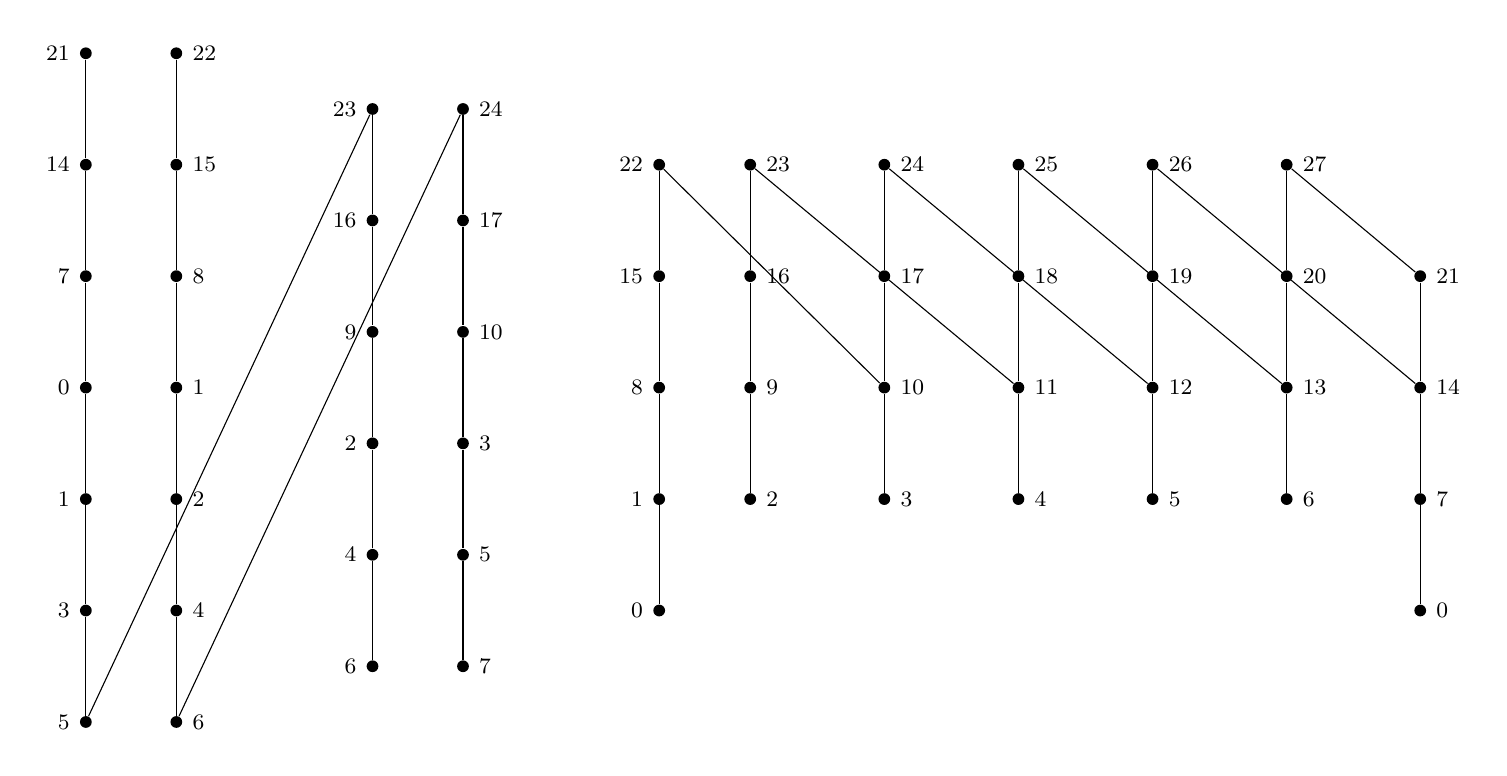
\begin{tikzpicture}[node distance=1cm and 1cm,
    dot/.style={circle, fill=black, inner sep=1.5pt},
    every label/.append style={font=\footnotesize},
    >=stealth
]

% LEFT DIAGRAM: {1^6, 7^{18}}
\matrix (grid) [row sep=1cm, column sep=1cm]
{
    \node [dot,label={left:$21$}] (a1) {}; & 
    \node [dot,label={right:$22$}] (a2) {}; \\
    \node [dot,label={left:$14$}] (b1) {}; & 
    \node [dot,label={right:$15$}] (b2) {}; \\
    \node [dot,label={left:$7$}] (c1) {}; &
    \node [dot,label={right:$8$}] (c2) {}; \\
    \node [dot,label={left:$0$}] (d1) {}; &
    \node [dot,label={right:$1$}] (d2) {}; \\
    \node [dot,label={left:$1$}] (e1) {}; &
    \node [dot,label={right:$2$}] (e2) {}; \\
    \node [dot,label={left:$3$}] (f1) {}; &
    \node [dot,label={right:$4$}] (f2) {}; \\
    \node [dot,label={left:$5$}] (g1) {}; &
    \node [dot,label={right:$6$}] (g2) {}; \\
};

% Connections within the left diagram
\draw (a1) -- (b1);
\draw (b1) -- (c1);
\draw (c1) -- (d1);
\draw (d1) -- (e1);
\draw (e1) -- (f1);
\draw (f1) -- (g1);

\draw (a2) -- (b2);
\draw (b2) -- (c2);
\draw (c2) -- (d2);
\draw (d2) -- (e2);
\draw (e2) -- (f2);
\draw (f2) -- (g2);

% RIGHT SIDE OF THE GRID
\matrix (grid2) [right=of grid, row sep=1cm, column sep=1cm]
{
    \node [dot,label={left:$23$}] (h1) {}; & 
    \node [dot,label={right:$24$}] (h2) {}; \\
    \node [dot,label={left:$16$}] (i1) {}; & 
    \node [dot,label={right:$17$}] (i2) {}; \\
    \node [dot,label={left:$9$}] (j1) {}; &
    \node [dot,label={right:$10$}] (j2) {}; \\
    \node [dot,label={left:$2$}] (k1) {}; &
    \node [dot,label={right:$3$}] (k2) {}; \\
    \node [dot,label={left:$4$}] (l1) {}; &
    \node [dot,label={right:$5$}] (l2) {}; \\
    \node [dot,label={left:$6$}] (m1) {}; &
    \node [dot,label={right:$7$}] (m2) {}; \\
};

% Connections within the right diagram
\draw (h1) -- (i1);
\draw (i1) -- (j1);
\draw (j1) -- (k1);
\draw (k1) -- (l1);
\draw (l1) -- (m1);

\draw (h2) -- (i2);
\draw (i2) -- (j2);
\draw (j2) -- (k2);
\draw (k2) -- (l2);
\draw (l2) -- (m2);

% CONNECTING NODES BETWEEN LEFT AND RIGHT
\draw (g1) -- (h1);
\draw (g2) -- (h2);

% RIGHT DIAGRAM: {1^7, 7^{17}, 8^3}
\matrix (spread) [right=of grid2, row sep=1cm, column sep=1cm]
{
    \node [dot,label={left:$22$}] (n1) {}; & 
    \node [dot,label={right:$23$}] (n2) {}; &
    \node [dot,label={right:$24$}] (n3) {}; &
    \node [dot,label={right:$25$}] (n4) {}; &
    \node [dot,label={right:$26$}] (n5) {}; &
    \node [dot,label={right:$27$}] (n6) {}; \\
    \node [dot,label={left:$15$}] (o1) {}; & 
    \node [dot,label={right:$16$}] (o2) {}; &
    \node [dot,label={right:$17$}] (o3) {}; &
    \node [dot,label={right:$18$}] (o4) {}; &
    \node [dot,label={right:$19$}] (o5) {}; &
    \node [dot,label={right:$20$}] (o6) {}; &
    \node [dot,label={right:$21$}] (o7) {}; \\
    \node [dot,label={left:$8$}] (p1) {}; &
    \node [dot,label={right:$9$}] (p2) {}; &
    \node [dot,label={right:$10$}] (p3) {}; &
    \node [dot,label={right:$11$}] (p4) {}; &
    \node [dot,label={right:$12$}] (p5) {}; &
    \node [dot,label={right:$13$}] (p6) {}; &
    \node [dot,label={right:$14$}] (p7) {}; \\
    \node [dot,label={left:$1$}] (q1) {}; &
    \node [dot,label={right:$2$}] (q2) {}; &
    \node [dot,label={right:$3$}] (q3) {}; &
    \node [dot,label={right:$4$}] (q4) {}; &
    \node [dot,label={right:$5$}] (q5) {}; &
    \node [dot,label={right:$6$}] (q6) {}; &
    \node [dot,label={right:$7$}] (q7) {}; \\
    \node [dot,label={left:$0$}] (r1) {}; & 
    &&&&& 
    \node [dot,label={right:$0$}] (r7) {}; \\
};

% Connections within the right diagram
\draw (n1) -- (o1);
\draw (n2) -- (o2);
\draw (n3) -- (o3);
\draw (n4) -- (o4);
\draw (n5) -- (o5);
\draw (n6) -- (o6);

\draw (o1) -- (p1);
\draw (o2) -- (p2);
\draw (o3) -- (p3);
\draw (o4) -- (p4);
\draw (o5) -- (p5);
\draw (o6) -- (p6);
\draw (o7) -- (p7);

\draw (p1) -- (q1);
\draw (p2) -- (q2);
\draw (p3) -- (q3);
\draw (p4) -- (q4);
\draw (p5) -- (q5);
\draw (p6) -- (q6);
\draw (p7) -- (q7);

\draw (q1) -- (r1);
\draw (q7) -- (r7);

% Additional diagonal connections in the right diagram
\draw (n1) -- (p3);
\draw (n2) -- (p4);
\draw (n3) -- (p5);
\draw (n4) -- (p6);
\draw (n5) -- (p7);
\draw (n6) -- (o7);

\end{tikzpicture}

\end{document}